\documentclass[11pt]{article}

\usepackage[margin = 1.0in]{geometry}
\usepackage[spanish]{babel}
\usepackage{setspace}
\onehalfspacing
\usepackage{here}
\usepackage{amsmath}
\usepackage{amssymb}
\usepackage{mathtools}
\usepackage{bm}
\usepackage{enumitem}
\usepackage{sectsty}
\usepackage{graphicx}
\usepackage[colorlinks=true,urlcolor=blue]{hyperref}
\usepackage{authblk}
\usepackage{caption}
\usepackage{fancyvrb}
\usepackage{relsize}
\usepackage{minted}
\usepackage{verbatim}
\usepackage{subcaption}
\usepackage{multirow}

\renewcommand\Authand{, }
\renewcommand\Authands{, }

\title{Inteligencia Artificial Generativa - Obligatorio 1}
\author{Matias Molinolo}
\author{Martina Diaz}
\affil{Facultad de Ingeniería, Universidad ORT Uruguay}

\date{\today}

\begin{document}
\maketitle
\begin{center}
    \url{https://github.com/matiasmolinolo/iag-2023}
\end{center}
\thispagestyle{empty}
\newpage
\tableofcontents
\newpage

\section{Estimación de distribuciones}

\subsection{Dataset 1: Tennis}
El objetivo fue estimar distribuciones de probabilidad a partir de un dataset `Tennis' con datos discretos. Inicialmente se calculó la probabilidad conjunta $p(x,y)$ y las probabilidades condicionales $p(y|x)$ y $p(x|y)$, siendo $x$ la variable discreta `Outlook' e $y$ la variable booleana `Tennis'. 

En segundo lugar buscamos aproximar $p(y,o,h,w,t)$ a través de la ecuación $p(y,o,h,w,t) = p(y) \times p(o|y) \times p(h|y,o) \times p(w|y,o) \times p(t|y,o,h,w)$. Para ello agrupamos las columnas necesarias del dataset y contabilizamos las ocurrencias de cada valor utilizando las funciones \texttt{groupby} y \texttt{size} de pandas DataFrame. Como resultado, observamos una probabilidad uniforme para las combinaciones de $(y,o,h,w,t)$ que aparecen en el dataset, lo cual se debe a que los datos provistos contienen como máximo una única ocurrencia cada combinación, por lo que la probabilidad de todos los casos posibles es $0$ o $0.071429$.

\begin{table}[h]
\centering
\begin{tabular}{c|c|c|c|c||c}
Outlook                   & Tennis               & Humidity                & Wind                  & Temp & Probability \\ \hline \hline
\multirow{4}{*}{Overcast} & \multirow{4}{*}{Yes} & \multirow{2}{*}{High}   & Strong                & Mild & 0.071429    \\ \cline{4-6} 
                          &                      &                         & Weak                  & Hot  & 0.071429    \\ \cline{3-6} 
                          &                      & \multirow{2}{*}{Normal} & Strong                & Cool & 0.071429    \\ \cline{4-6} 
                          &                      &                         & Weak                  & Hot  & 0.071429    \\ \hline
\multirow{5}{*}{Rain}     & \multirow{2}{*}{No}  & High                    & Strong                & Mild & 0.071429    \\ \cline{3-6} 
                          &                      & Normal                  & Strong                & Cool & 0.071429    \\ \cline{2-6} 
                          & \multirow{3}{*}{Yes} & High                    & Weak                  & Mild & 0.071429    \\ \cline{3-6} 
                          &                      & \multirow{2}{*}{Normal} & \multirow{2}{*}{Weak} & Cool & 0.071429    \\ \cline{5-6} 
                          &                      &                         &                       & Mild & 0.071429    \\ \hline
\multirow{5}{*}{Sunny}    & \multirow{3}{*}{No}  & \multirow{3}{*}{High}   & Strong                & Hot  & 0.071429    \\ \cline{4-6} 
                          &                      &                         & \multirow{2}{*}{Weak} & Hot  & 0.071429    \\ \cline{5-6} 
                          &                      &                         &                       & Mild & 0.071429    \\ \cline{2-6} 
                          & \multirow{2}{*}{Yes} & \multirow{2}{*}{Normal} & Strong                & Mild & 0.071429    \\ \cline{4-6} 
                          &                      &                         & Weak                  & Cool & 0.071429   

    \end{tabular}
    \caption{Probabilidad conjunta $p(y,o,h,w,t)$}
    \label{tab:joint_proba_yohwt}
\end{table}

\subsection{Dataset 2: Iris}
marti

\newpage

\section{Modelos generativos}
\subsection{NADE: Neural Autoregressive Distribution Estimator}

Intentamos reproducir en Pytorch la arquitectura del NADE propuesta por \cite{nade}, con ciertas modificaciones que resultaron de la prueba y error de la arquitectura.

Uria et al. propone una arquitectura autorregresiva que parte de la base que cualquier distribución $D$-dimensional $p$ puede expresarse como un producto de distribuciones unidimensionales \cite{nade}:
$$
p(\boldsymbol{x}) = \prod_{d=1}^{D}p(x_{o_d} | \boldsymbol{x}_{o_{<d}})
$$

Para ello, nos basamos en el siguiente repositorio de Github: \url{https://github.com/simonjisu/NADE-pytorch/blob/master/model.py}, pero con ciertas modificaciones para la optimización de los cálculos.

Nuestra arquitectura usa 192 unidades ocultas, en vez de las 500 propuestas en el paper original. Esto se debe a que tras varios ensayos, encontramos que este número daba una buena performance y un tiempo de ejecución significativamente menor al de la arquitectura original del paper. 

El NADE fue entrenado con datos binarizados del dataset MNIST, donde se filtraron todos aquellos elementos que no pertenecían a la clase que quería generarse.

Podemos ver el código de la función \texttt{forward} del NADE a continuación:

\begin{minted}{python3}
    a = self.c.expand(x.shape[0], -1)

    p_x_hat = []

    for d in range(self.input_dim):
        h_d = torch.sigmoid(a)
        p = torch.sigmoid(h_d @ self.V[d:d+1, :].t() + self.b[d:d+1])
        p_x_hat.append(p)
        a = x[:, d:d+1] @ self.W[:, d:d+1].t() + a

    probs = torch.cat(p_x_hat, 1)
    return probs
\end{minted}

Luego de entrenarlo por 50 epochs, donde alcanzamos una loss de $0.29$, hicimos un muestreo de la distribución estimada por el NADE con el siguiente código:
\begin{minted}{python3}
    with torch.no_grad():
    preds = torch.zeros(1, input_dim).to(device)
    for i in tqdm(range(input_dim)):
        p = model.forward(preds)
        preds[0][i] = torch.bernoulli(p[0][i])

    return torch.reshape(preds.cpu(), (28, 28))
\end{minted}
Donde obtuvimos el siguiente resultado:

\begin{figure}[h]
    \centering
    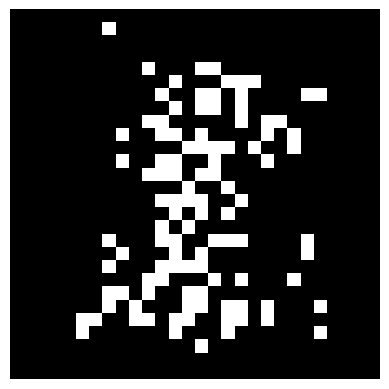
\includegraphics[width=0.6\textwidth]{NADE/nade_generation.png}
    \caption{Distribución estimada por el NADE}
    \label{fig:nade_gen}
\end{figure}

Podemos ver que no es una representación totalmente acertada, pero se puede apreciar claramente que se asemeja a la clase original de los 1. Estimamos que esto puede deberse a falta de entrenamiento u otros factores.
\newpage
\subsection{VAE: Variational Autoencoder}

A partir del tutorial de Doersch \cite{vae}, entrenamos un VAE y un VAE condicional, es decir, que genera una nueva imagen dada una clase específica.

Nuevamente, entrenamos esta red con el dataset del MNIST, pero esta vez sin filtrar ni binarizar.

Es interesante visualizar el espacio latente del VAE y el VAE condicional, que podemos observar en las siguientes figuras:

\begin{figure}[h]
\begin{subfigure}[h]{0.5\linewidth}
    \centering
    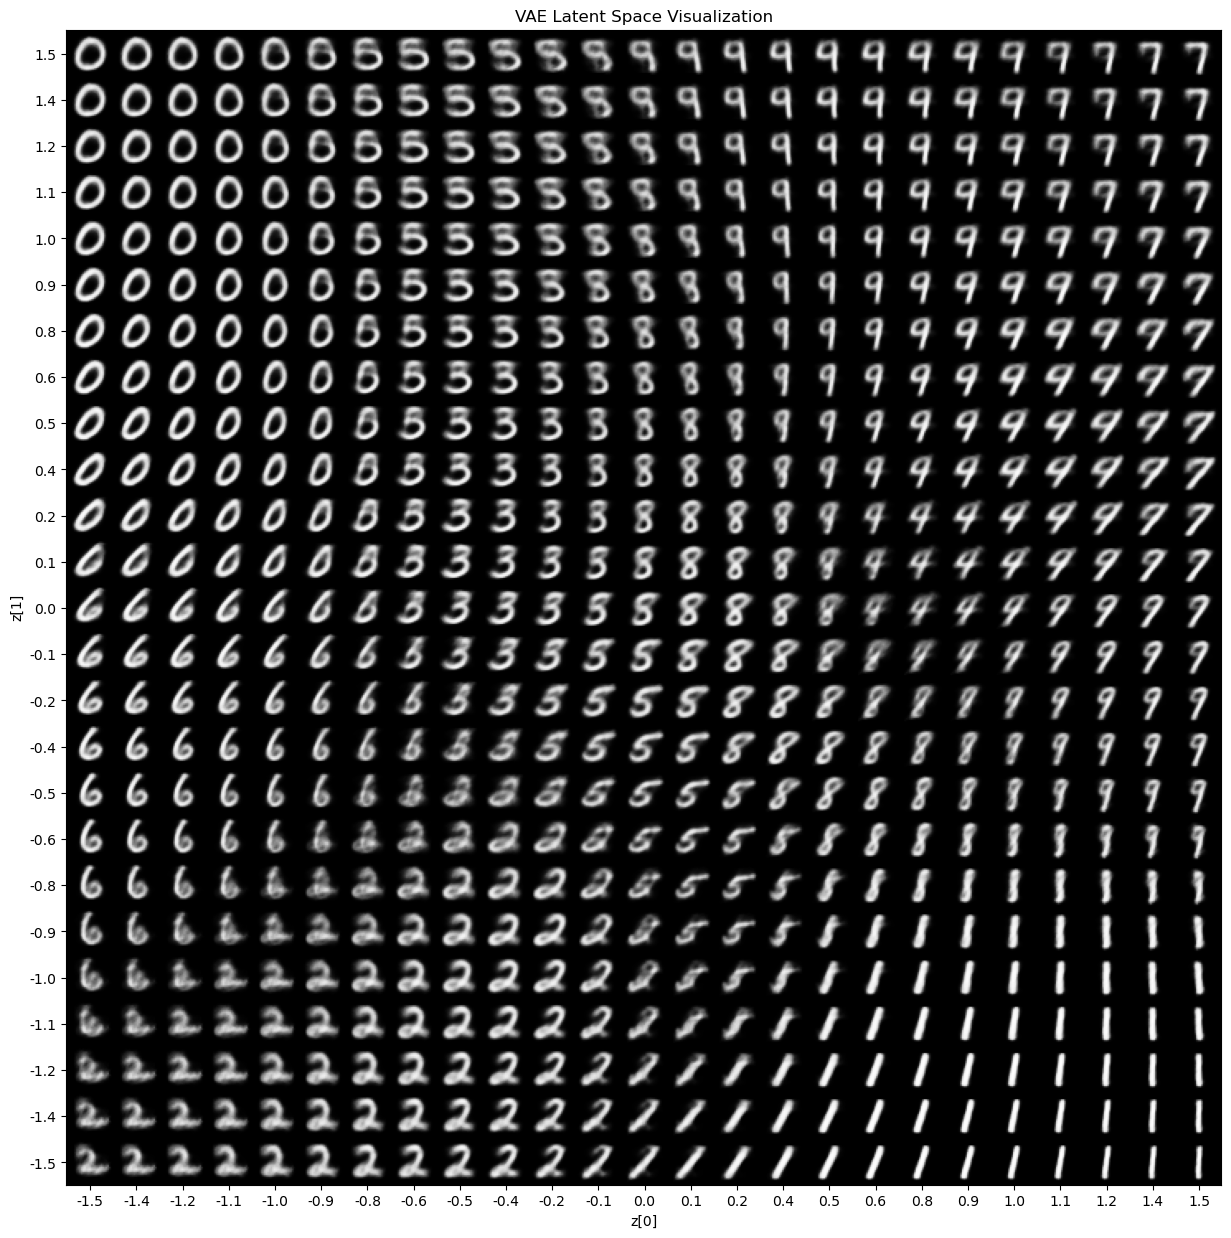
\includegraphics[width=\linewidth]{VAE/latent_space_vae.png}
    \caption{Espacio latente del VAE}
    \label{fig:vae_latent_space}
\end{subfigure}
\begin{subfigure}[h]{0.5\linewidth}
    \centering
    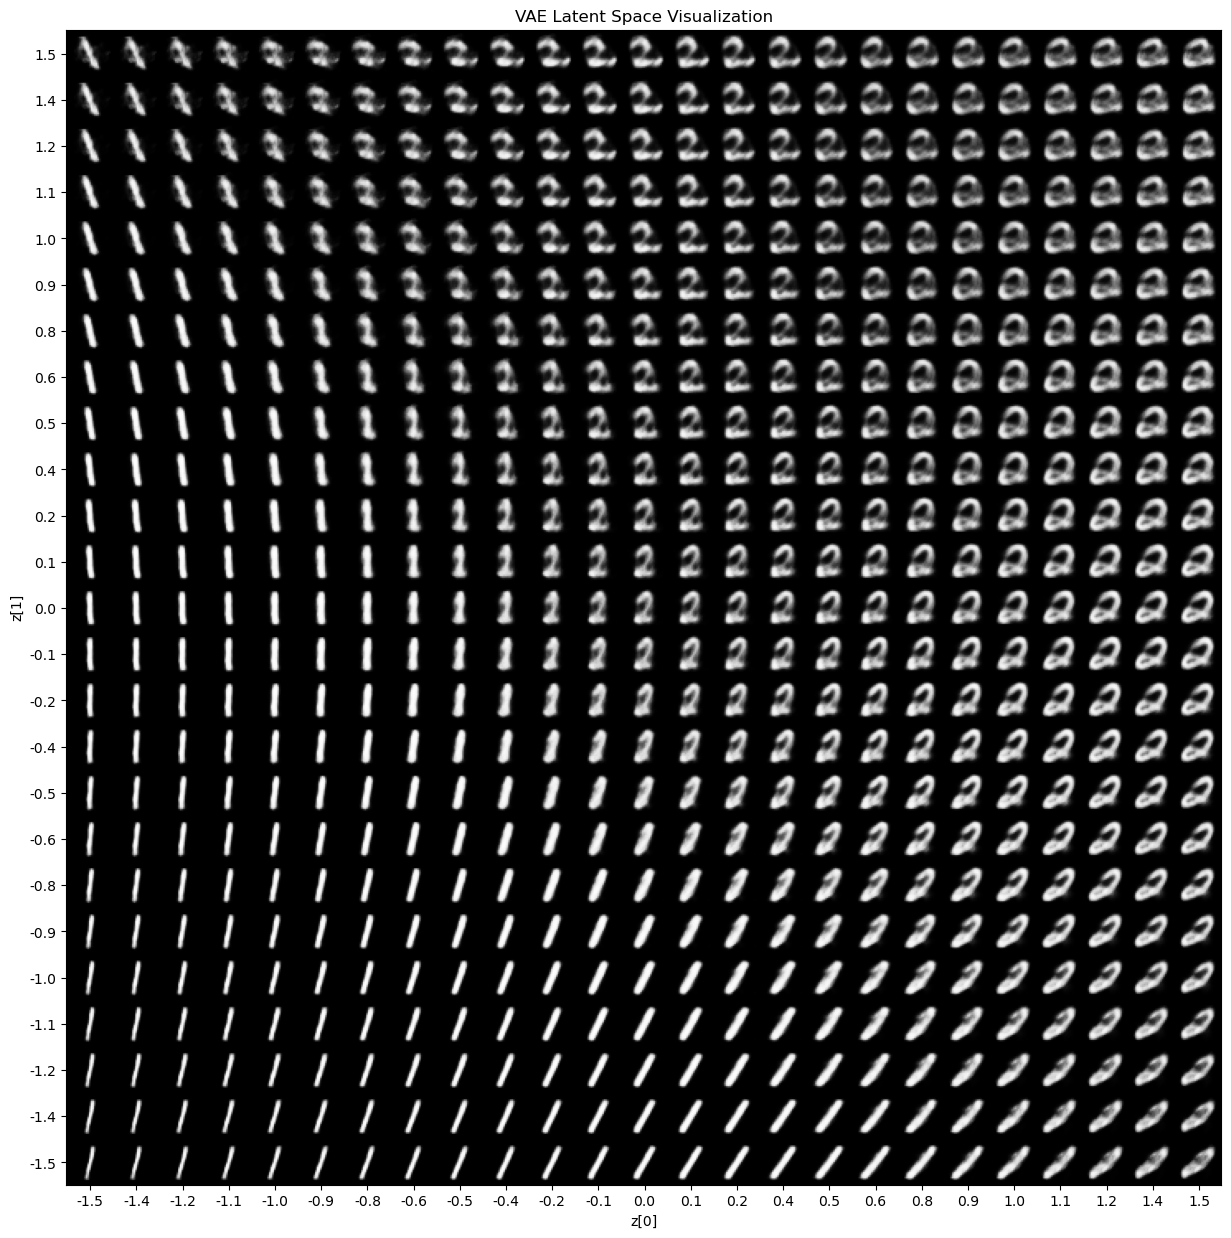
\includegraphics[width=\linewidth]{VAE/latent_space_cvae.png}
    \caption{Espacio latente del VAE condicional}
    \label{fig:cvae_latent_space}
\end{subfigure}
\end{figure}

Podemos apreciar como en el espacio latente del VAE se generan nuevas imágenes que se asemejan a todas las clases del dataset, mientras que en el espacio latente del VAE condicional se generan nuevas imágenes acotadas a la clase que indicamos como condicional.

A diferencia del NADE, tanto el entrenamiento como el sampling del VAE es mucho más rápido y genera mejores resultados en menos epochs - esto se debe al carácter autorregresivo del NADE, que hace imposible su paralelización, a diferencia del VAE que si es paralelizable.
\newpage

\bibliographystyle{ieeetr}
\bibliography{refs}

\end{document}
